\section{Results and discussion}

\subsection{Thorium feed mechanism}

The first mechanism adopts continuous feed flow of external thorium and $^{233}$U from Pa-decay tank. Hereinafter the first mechanism will be mentioned as the thorium feed mechanism. The molar fraction of the heavy metal in the initial fuel was kept constant and equal to 12.5 mole\% for all cases. Besides, the initial fissile material fraction was increased for the five fuel salt compositions until the SD-TMS reactor was sufficiently critical at the Beginning Of Life (BOL). 
Figure~\ref{fig:keff1} illustrates the change of the effective multiplication with \gls{EFPY} for the thorium feed mechanism.
As shown in Figure~\ref{fig:keff1}, the effective multiplication factor ($k_{eff}$) decreases sharply during the first 25 years of reactor operation for the first four cases. $k_{eff}$ decreases as a result of depletion of the initial fissile materials and generation of the neutron poisons (FPs). Thus, the reactor becomes subcritical within a relatively short time ($\approx$ $4$ $years$ in the \gls{TRU} case and $\approx$ $12$ $years$ in the Pu reactor-grade case). The amount of $^{233}$U generated in the \gls{SD-TMSR} is not enough to conserve the reactor criticality and overcome the neutron absorption in the initial fertile isotopes.
Nevertheless, the continuous feed flow of thorium and $^{233}$U helps to operate the \gls{SD-TMSR} for a long period of time (the U-233 case). Besides, the initial molar fraction of LEU and Pu reactor-grade was increased more (Figure~\ref{fig:keff1}) to counteract the absorption of neutrons in the non-fissile heavy metals added with the initial fuel salt. But $k_{eff}$ still decreases below 1.0, as a result of increasing the non-fissile heavy metals in the initial fuel \cite{betzler2016modeling}.

\begin{figure}
	\centering
	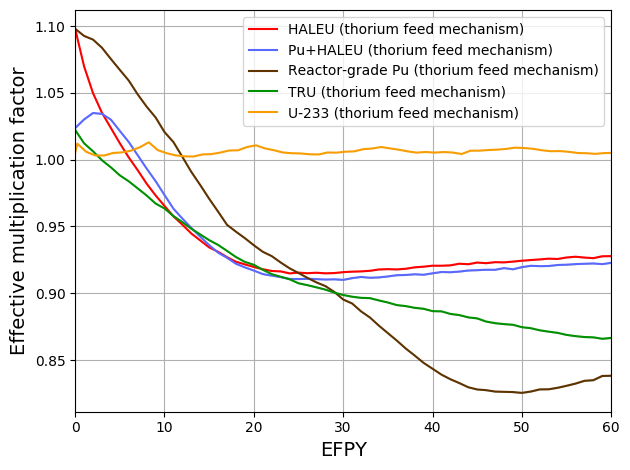
\includegraphics[width=\textwidth]{keff1.png}
	\caption{The change of the effective multiplication factor during 60 \gls{EFPY} of reactor operation for thorium feed mechanism (confidence interval $\pm\sigma$ is shaded).} 
	\label{fig:keff1}
\end{figure}

\subsection{Non-thorium feed mechanism}

The second mechanism allows continuous feed flow of $^{233}$U only from Pa-decay tank and the same composition of the initial fuel except for thorium. Hereinafter the second mechanism will be mentioned as the non-thorium feed mechanism. Figure~\ref{fig:keff2} shows the change of the effective multiplication during 60 \gls{EFPY} of reactor operation for the non-thorium feed mechanism.
As shown in Figure~\ref{fig:keff2}, the SD-TMS reactor was sufficiently critical at the Beginning Of Life (BOL). Both Pu reactor-grade and TRU case show good results relative to the other two cases (i.e. LEU and Pu+LEU). For the Pu reactor-grade fuel salt, the amount of $^{233}$U generated in the \gls{SD-TMSR} in addition to the external feed flow of Pu are sufficient to maintain the reactor criticality and overcome the neutron absorption in the initial non-fissile isotopes. This may be attributed to the fact that the spectrum in the Pu reactor-grade initial core is hardened that is more thorium is being converted to $^{233}$U. For the \gls{TRU} fuel salt, the amount of $^{233}$U and the external feed flow of TRU is barely enough to operate the reactor for a long period of time ($\approx$ $40$ $years$) without any external feed of $^{233}$U. Nevertheless, $k_{eff}$ decreases with the burnup time because the minor actinides accumulating in the core as a result of continuous TRU feed. As shown in Figure~\ref{fig:keff2}, the LEU and Pu+LEU fuel are less attractive for non-thorium feed mechanism. The continuous LEU feed increases the amount of fertile $^{238}$U and consequently, reduces the feasibility of such fissile materials. The continuous feed of $^{233}$U without $^{232}$Th will lead to supercritical reactor, thus the $^{233}$U case is excluded from non-thorium feed mechanism.\\
According to the $k_{eff}$ results, Pu reactor-grade and TRU fissile materials are selected and discussed in the following. 
\begin{figure}
	\centering
	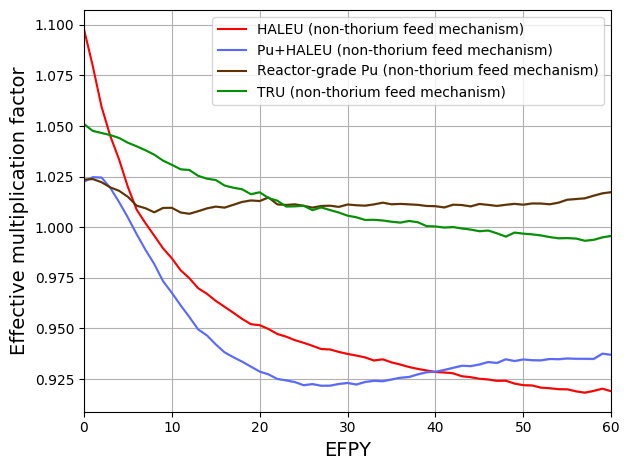
\includegraphics[width=\textwidth]{keff2.png}
	\caption{The change of the effective multiplication factor during 60 \gls{EFPY} of reactor operation for non-thorium feed mechanism (confidence interval $\pm\sigma$ is shaded).} 
	\label{fig:keff2}
\end{figure}

\subsection{Pu reactor-grade, TRU, and $^{233}$U initial fuel}

In this section, the simulation of the SD-TMSR with Pu reactor-grade and TRU fissile materials is discussed. Besides, the $^{233}$U case is listed for comparison.\\
Figure~\ref{fig:refillCCC} demonstrates the dynamics of heavy metal refill rate during 60 \gls{EFPY} of SD-TMSR operation. The heavy metal refill rate was adjusted to maintain; the reactor criticality and total fuel mass almost constant (less than $0.1\%$) during the reactor operation. In $^{233}$U case, the mean values of $^{233}$U and $^{232}$Th refill rate are $1.77$ and $2.21$ $kg/d$, respectively. As well, in the Pu reactor-grade case, the mean values of $^{233}$U and Pu refill rate are $0.75$ and $2.75$ $kg/d$, respectively. In the TRU case, the mean values of $^{233}$U and TRU refill rate are $0.90$ and $2.0$ $kg/d$, respectively.

\begin{figure}
	\centering
	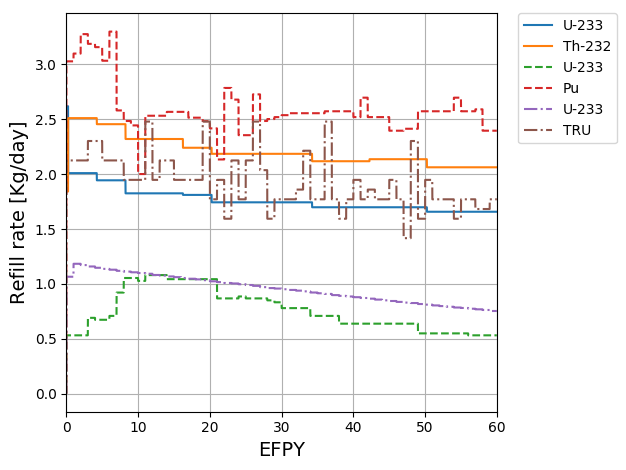
\includegraphics[width=\textwidth]{refillCCC.png}
	\caption{Dynamics of heavy metal refill rate during 60 \gls{EFPY} of reactor operation. Solid lines for $^{233}$U case, dashed lines for Pu reactor-grade case, and dotted lines for TRU case.}
	\label{fig:refillCCC}
\end{figure}

Figure~\ref{fig:inventoryCCCC} and ~\ref{fig:inventoryPu_TRUCCC} describe the evolution of important isotopes for $^{233}$U, Pu and TRU cases respectively.
From Figure~\ref{fig:inventoryCCCC}, The mass of Pa in the fuel salt is almost constant and reaches $17.8$ $kg$ at the end of the operation time. In addition, the mass of Minor Actinides\footnote{In the present work, the Minor Actinides (MA) include Np, Am and Cm.} (MA) increases with time; however, by applying online reprocessing, its value remains relatively low. As well, the total mass of Pu increases with burnup time. The level of Pu in the fuel correlates with the mass of the MA, and Pu. MA need more time to reach equilibrium. The total mass of U increases with burnup time and reaches equilibrium after $\approx$ $27$ $years$. As shown in Figure~\ref{fig:inventoryCCCC}, refueling the core with Th helps maintain an almost constant inventory throughout the full operation time.\\
The Pa extraction time was adjusted to be 30 seconds for Pu and TRU cases to avoid poisoning the core. Therefore, Figure~\ref{fig:inventoryPu_TRUCCC} shows that the mass of Pa in the fuel for Pu and TRU cases is relatively low when compared to the $^{233}$U case.
Major isotopes for the three cases reaches the equilibrium state after $\approx$ $30$ $years$ (see Figure~\ref{fig:inventoryCCCC} and ~\ref{fig:inventoryPu_TRUCCC}).

\begin{figure}
	\centering
	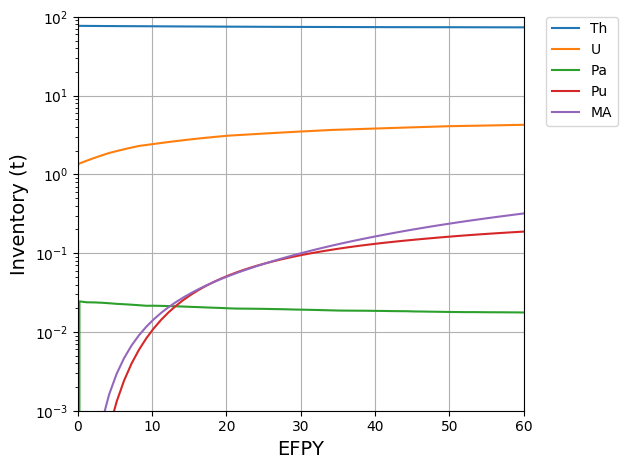
\includegraphics[width=\textwidth]{inventoryCCCC.png}
	\caption{Evolution of the important nuclides inventories for $^{233}$U case ($^{\star}$MA involves Np, Am, Cm).}
	\label{fig:inventoryCCCC}
\end{figure}

\begin{figure}
	\centering
	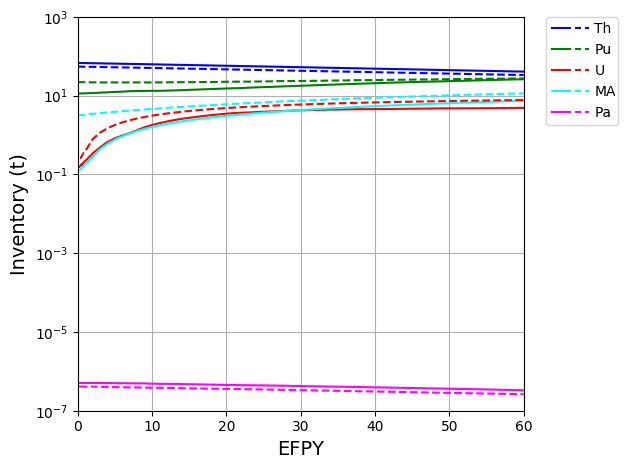
\includegraphics[width=\textwidth]{inventoryPu_TRUCCC.png}
	\caption{Evolution of the important nuclides inventories for Pu reactor-grade case (solid lines) and for TRU case (dashed lines).}
	\label{fig:inventoryPu_TRUCCC}
\end{figure}


Figure~\ref{fig:Th232CC} illustrates the variation of thorium mass in the fuel salt for $^{233}$U, Pu reactor-grade and TRU cases, respectively. In $^{233}$U case, we apply the thorium feed mechanism, thus thorium mass decreases by only $3.2$ $\%$ at the end of operation time (60 years). In contrast, thorium mass decreases significantly in Pu and TRU cases according to the non-thorium feed mechanism. Thorium mass decreases by $39.2$ $\%$ and $37.96$ $\%$ in Pu reactor-grade and TRU cases, respectively. The maximum decreasing in thorium mass refer to the effective utilization of thorium fuel cycle. Consequently, the Pu reactor-grade initial fuel may help to utilize thorium fuel cycle more effective.

\begin{figure}
	\centering
	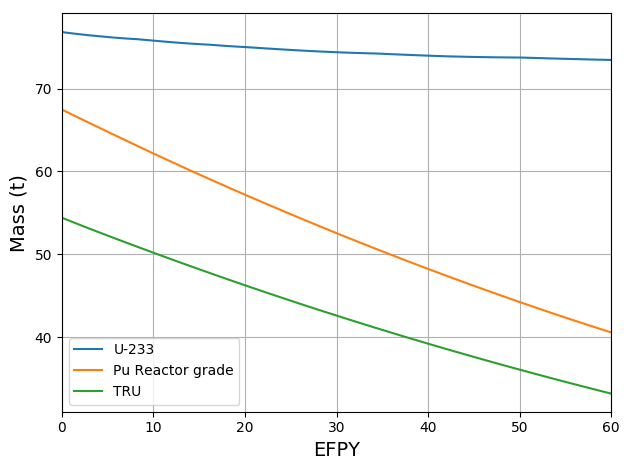
\includegraphics[width=\textwidth]{Th232CC.png}
	\caption{The variation of thorium mass in the fuel salt for $^{233}$U, Pu reactor-grade and TRU cases, respectively.}
	\label{fig:Th232CC}
\end{figure}

Figure~\ref{fig:U233CC} demonstrates the mass of $^{233}$U in the fuel salt for $^{233}$U, Pu reactor-grade and TRU cases, respectively. One can see that the mass of the $^{233}$U reaches the equilibrium state after $\approx$ $30$ $years$. Meanwhile, the amount of $^{233}$U is sufficient to maintain criticality in the three cases.

\begin{figure}
	\centering
	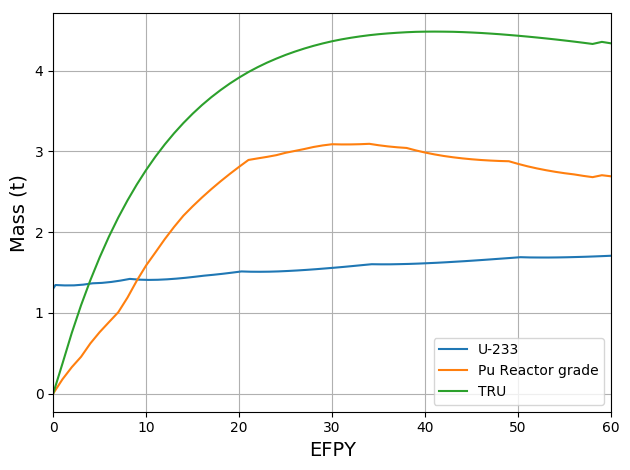
\includegraphics[width=\textwidth]{U233CC.png}
	\caption{Mass of $^{233}$U in the fuel salt for $^{233}$U, Pu reactor-grade and TRU case, respectively.}
	\label{fig:U233CC}
\end{figure}

In the non-thorium feed mechanism, the SD-TMSR is continuously refueled for criticality, which increases the Pu proportion in the molten salt. According to the literature, the limit of Pu solubility in the FLiBe salt is $\approx$ $4.0$ $\%$ \cite{ignatiev2012progress,sood1975plutonium}. Figure~\ref{fig:PusolubilityCC} represents the Pu proportion in the fuel salt (mole\%). In $^{233}$U and Pu reactor-grade cases, the Pu proportion increases slightly but still below its solubility limit. On the other hand, the Pu proportion in the molten salt loaded by TRU increases with operation time and exceeds the Pu solubility limit.
This issue may be solved by increasing the reactor operation temperature and or reducing the HM initial inventory \cite{zou2018transition}.

\begin{figure}
	\centering
	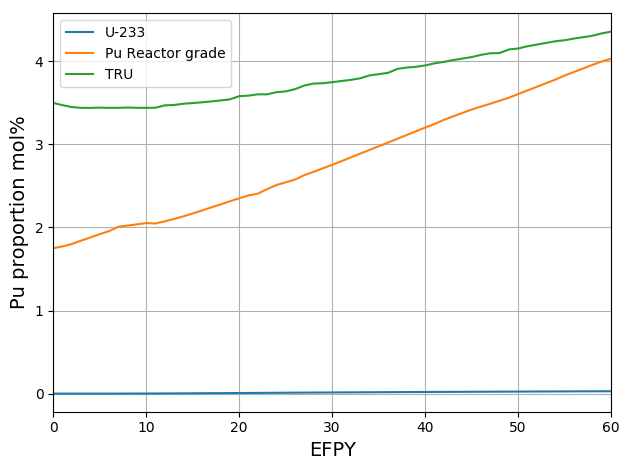
\includegraphics[width=\textwidth]{PusolubilityCC.png}
	\caption{The Pu proportion in the fuel salt (mole\%).}
	\label{fig:PusolubilityCC}
\end{figure}


Figure~\ref{fig:NetCC} demonstrates the net production of $^{233}$U as a function of burnup time. In TRU case, the net production of $^{233}$U is almost zero, nevertheless, the reactor becomes subcritical after 40 years of operation. In $^{233}$U and Pu reactor-grade cases, the net production of $^{233}$U increases with burnup time and reaches about $1.77$ $t$ and $10$ $t$, respectively at the end of operation lifetime. It worth noting that thorium feed mechanism is applied in $^{233}$U case, while, non-thorium feed mechanism is adopted in Pu reactor-grade cases.
As shown in Figure~\ref{fig:NetCC}, after 26 years the net production of $^{233}$U reaches $1.3$ $t$; this is sufficient to start-up another \gls{SD-TMSR}. Similarly, one can see that the same amount of $^{233}$U (i.e. $1.3$ $t$) can be achieved after $\approx$ $4.5$ $years$ if we applied the non-thorium feed mechanism on the SD-TMSR that initially loaded by Pu reactor-grade alternative to $^{233}$U. In addition, Figure~\ref{fig:NetCC} also shows that the net production of $^{233}$U during the first 455 days is negative, thus about $175.28$ $kg$ of $^{233}$U must be added during this period. In conclusion, the thorium fuel cycle transition can be achieved by selecting the proper feed mechanism and initial fissile material. 

\begin{figure}
	\centering
	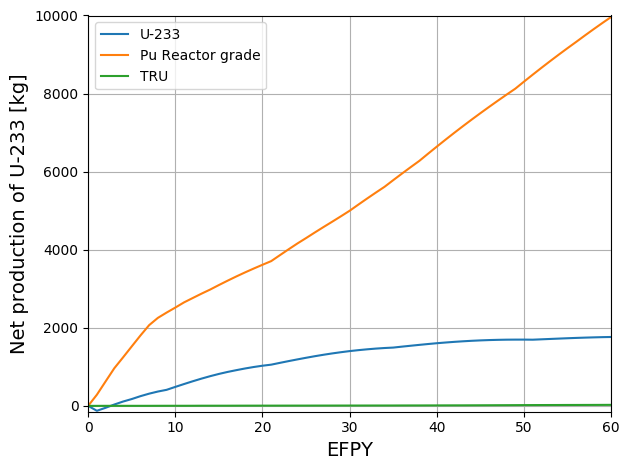
\includegraphics[width=\textwidth]{NetCC.png}
	\caption{Net production of $^{233}$U during burn-up period (60 \gls{EFPY}).}
	\label{fig:NetCC}
\end{figure}

\subsection{Neutron spectrum}

Figure~\ref{fig:spectrumFLUX110vC} represents the normalized neutron flux spectrum for full-core SD-TMSR model in the energy range from 10$^{-8}$ to 10 MeV for the $^{233}$U, Pu reactor-grade, and TRU started case. In $^{233}$U case, at the EOL, the neutron spectrum is harder than at BOL due to the accumulation of the Pu and other strong thermal neutron absorbers in the fuel salt. In Pu reactor-grade and TRU cases and during the reactor operation, the fissile Pu is depleted and the $^{233}$U becomes the major fissile isotope, the neutron spectrum softens and becomes similar to a thermal spectrum of the TMSR.
 
 
\begin{figure}
 	\centering
 	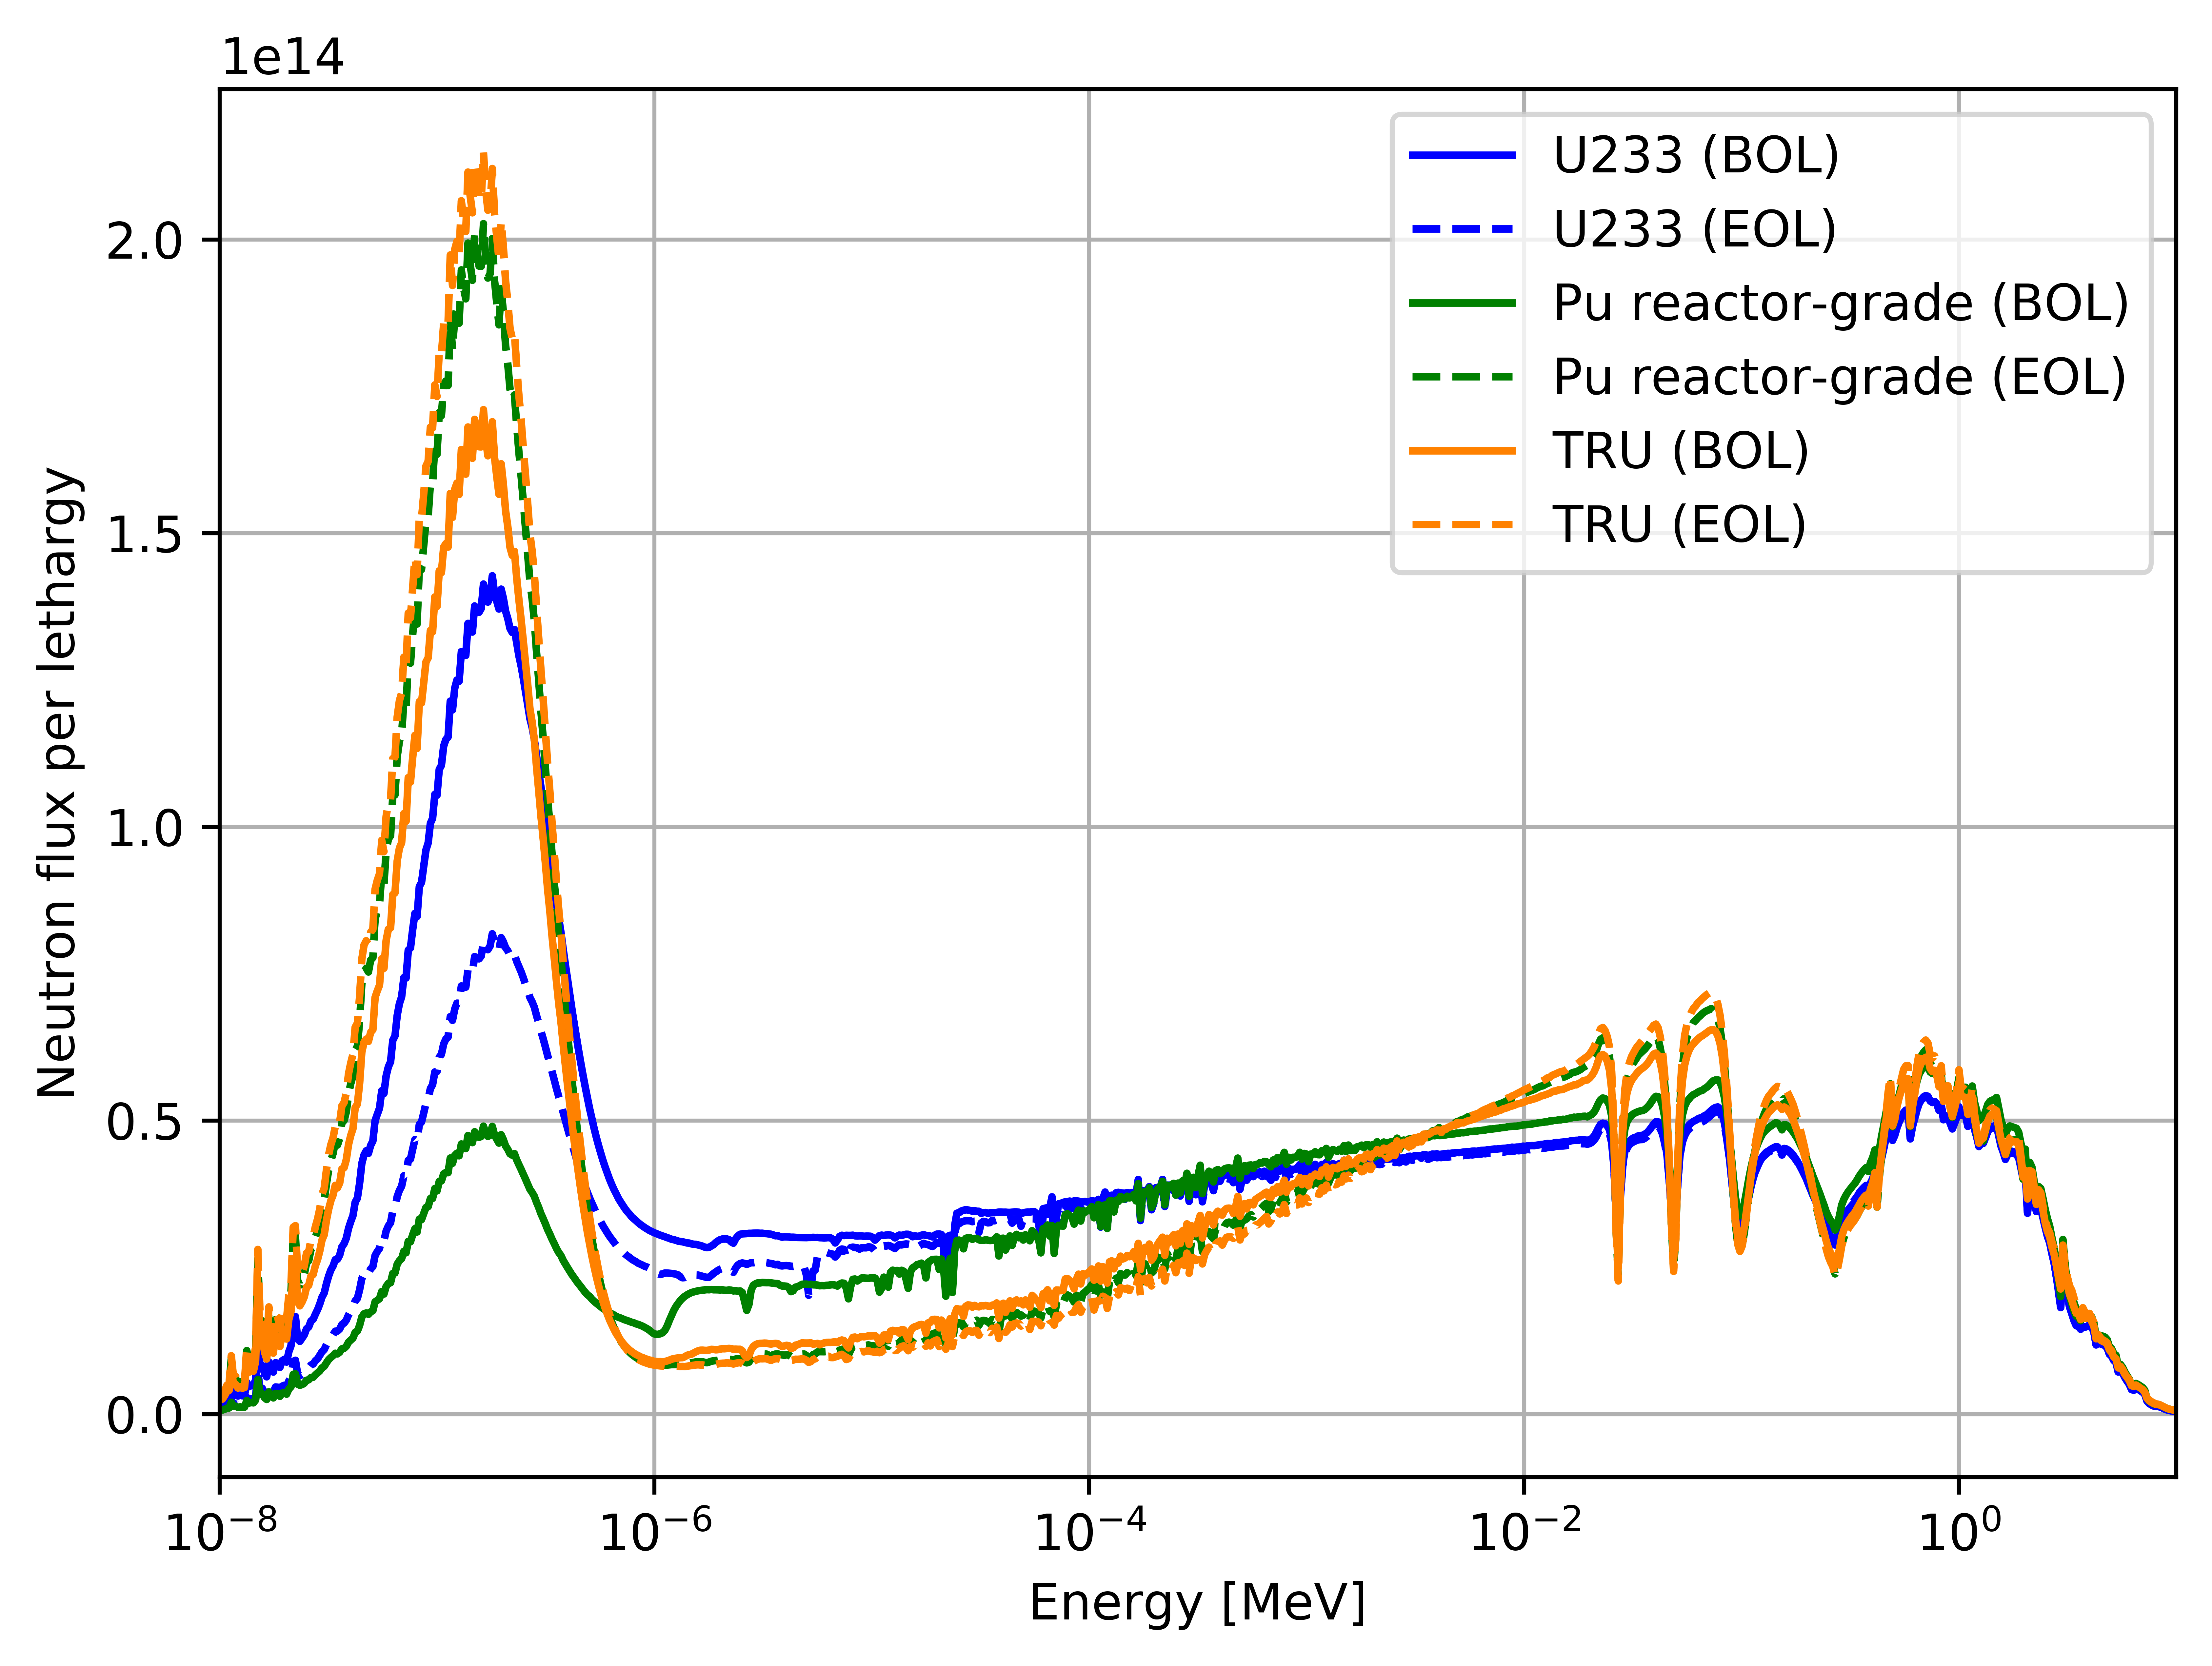
\includegraphics[width=\textwidth]{spectrumFLUX110vC.png}
 	\caption{The neutron flux energy spectrum at different BOL (solid lines) and EOL (dashed lines).}
 	\label{fig:spectrumFLUX110vC}
\end{figure}


The comparison of the two feed mechanisms based on five different types of initial fuel is listed in Table~\ref{tab:table7}. 
	
	
\begin{table} % [!ht]
	\centering
	\caption{Comparison of the two feed mechanisms based on five different types of initial fuel.}
	\vspace{0.1in}
	\begin{tabularx}{\textwidth}{s s s s s s }  %{\textwidth}
		\hline
		\backslashbox{Feed mechanism}{Initial fuel}& \gls{LEU} (19.79\%) & Pu mixed with enriched U (19.79 wt-\%) & Pu reactor-grade & \gls{TRU}& $^{233}$U \\
		\hline
		Thorium feed mechanism&Not work&Not work&Not work&Not work& Work\\
		Non-thorium feed mechanism &Not work&Not work&Work well with positive net production of $^{233}$U &Work for 40 years with net production of $^{233}$U = zero & Not examine (supercritical reactor)\\
		\hline
	\end{tabularx}
	\label{tab:table7}
\end{table}
